\section{Base de dados}
A base de dados fornecida estava, inicialmente, separada em 2 arquivos, adult\_test e adult\_data, aos quais adicionou-se uma linha de cabeçalho para importação no Matlab, unificou-se ambos arquivos para o pré-processamento. A base de dados é composta por 14 atributos e 1 atributo-alvo, que representa se a renda é inferior a 50 mil dólares anuais ou igual ou superior a 50 mil dólares anuais, sendo eles:

\begin{description}
\item[Age] \hfill \\ Atributo contínuo que representa idade;
\item[Workclass] \hfill \\ Atributo categórico que representa uma das 9 classes de trabalho;
\item[Fnlwgt] \hfill \\ Atributo contínuo;
\item[Education] \hfill \\ Atributo categórico que representa um dos 16 graus de escolaridade;
\item[Education-num] \hfill \\ Atributo continuo relacionado ao grau de escolaridade;
\item[Marital-status] \hfill \\ Atributo categórico que representa um dos 7 estados civis;
\item[Occupation] \hfill \\ Atributo categórico que representa uma das 14 áreas de trabalho;
\item[Relationship] \hfill \\ Atributo categórico que representa um dos 6 parentescos;
\item[Race] \hfill \\ Atributo categórico que representa uma das 5 etnias;
\item[Sex] \hfill \\ Atributo categórico que representa um dos 2 sexos possíveis;
\item[Capital-gain] \hfill \\ Atributo contínuo que representa o ganho de capital;
\item[Capital-loss] \hfill \\ Atributo contínuo que representa a perda de capital;
\item[Hours-per-week] \hfill \\ Atributo continuo que representa as horas trabalhadas por semana;
\item[Native-country] \hfill \\ Atributo categórico que representa um das 41 nacionalidades.
\end{description}

Após o carregamento removeu-se as amostras duplicadas, resultando em um total de 48813 amostras únicas, removeu-se também amostras com atributos idênticos porém com atributo-alvo distinto, resultando em 48785 amostras.

Apresentaram-se 3615 amostras com informações ausentes para os atributos: \textbf{work-class, occupation, native-country}. Essas amostras representavam cerca de 8\% do total, portanto, optou-se por removê-las da base dados. Resultando em 45170 amostras.

Os atributos contínuos não sofreram modificações para os métodos do KNN, Regressão Logística, Redes Neurais e SVM, entretanto para o método Naive Bayes discretizou-se os valores em 10 cestas e aplicou-se a suavização de Laplace a fim de tratar cestas que não continham valores.

Os atributos categóricos foram convertidos em colunas, sendo que cada coluna representa um dos valores possíveis para o atributo original e o valor de cada uma das colunas passa a ser binário, indicando se a categoria do atributo original é a representada pela coluna.

Devido a expansão dos atributos categóricos, 3 colunas representavam atributos ausentes para 3 atributos originais. Devido à remoção das amostras com atributos ausentes, tornou-se irrelevante manter essas colunas, portanto as mesmas foram removidas. Após essas transformações os 14 atributos originais tornaram-se 105. Para o método Naive-Bayes os 14 atributos originais tornaram-se 160.

O atributo-alvo foi convertido em um atributo binário, 1 para representar a classe positiva (renda igual ou superior a 50 mil dolares anuais) e 0 para representar a classe negativa (renda inferior a 50 mil dolares anuais). 11197 amostras (24,79\%) representam a classe positiva e 33973 amostras representam a classe negativa (75,21\%).

Implementou-se 2 tipos de normalização para todos os atributos, exceto o atributo-alvo:

\begin{description}
\item[Normalização por reescala] \hfill \\ Restringe o intervalo de valores entre 0 e 1 para um atributo, mais sensível a outliers;
\item[Normalização por padronização] \hfill \\ Garante que os valores tenham média igual a 0 e desvio-padrão igual a 1.
\end{description}

Para se permitir a visualizção dos dados, implementou-se a Análise de componentes principais (PCA), para redução dos 105 atributos para 3, resultando na imagem disposta na Figura \ref{fig:dados3d}, na qual a classe positiva, renda igual ou superior a 50 mil dólares anuais, é representada por \textcolor{blue}{+} e a classe negativa, renda inferior a 50 mil dólares anuais, é representada por \textcolor{red}{o}.

\begin{figure}[h]
\centering
\makebox[\columnwidth]{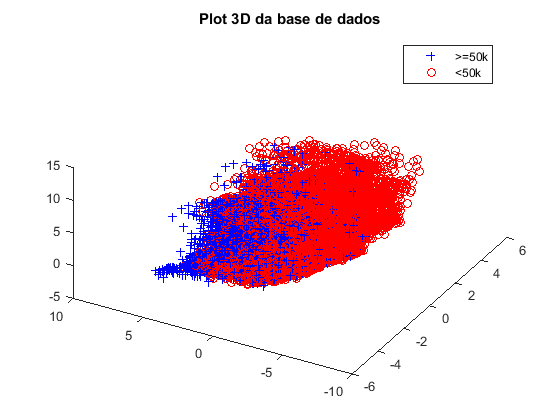
\includegraphics[width=\columnwidth]{dados3d}}
\caption{Plot 3D dos atributos}
\label{fig:dados3d}
\end{figure}